%%%%%%%%%%%%%%%%%%%%%%%%%%%%%%%%%%%%%%%%%
% University Assignment Title Page 
% LaTeX Template
% Version 1.0 (27/12/12)
%
% This template has been downloaded from:
% http://www.LaTeXTemplates.com
%
% Original author:
% WikiBooks (http://en.wikibooks.org/wiki/LaTeX/Title_Creation)
%
% License:
% CC BY-NC-SA 3.0 (http://creativecommons.org/licenses/by-nc-sa/3.0/)
% 
% Instructions for using this template:
% This title page is capable of being compiled as is. This is not useful for 
% including it in another document. To do this, you have two options: 
%
% 1) Copy/paste everything between \begin{document} and \end{document} 
% starting at \begin{titlepage} and paste this into another LaTeX file where you 
% want your title page.
% OR
% 2) Remove everything outside the \begin{titlepage} and \end{titlepage} and 
% move this file to the same directory as the LaTeX file you wish to add it to. 
% Then add \input{./title_page_1.tex} to your LaTeX file where you want your
% title page.
%
%%%%%%%%%%%%%%%%%%%%%%%%%%%%%%%%%%%%%%%%%
%\title{Title page with logo}
%----------------------------------------------------------------------------------------
%	PACKAGES AND OTHER DOCUMENT CONFIGURATIONS
%----------------------------------------------------------------------------------------
\documentclass[UTF-8,12pt]{article}
\usepackage[UTF8]{ctex}
\usepackage[english]{babel}
\usepackage[utf8x]{inputenc}
\usepackage{amsmath}
\usepackage{graphicx}
\usepackage[colorinlistoftodos]{todonotes}

\begin{document}

\begin{titlepage}

\newcommand{\HRule}{\rule{\linewidth}{0.5mm}} % Defines a new command for the horizontal lines, change thickness here

\center % Center everything on the page
 
%----------------------------------------------------------------------------------------
%	HEADING SECTIONS
%----------------------------------------------------------------------------------------

\textsc{\LARGE \bfseries 中山大学 }\\[0.3cm] % Name of your university/college
\textsc{\Large 数据科学与计算机学院}\\[0.5cm] % Major heading such as course name
\textsc{\Large 软件工程}\\[0.3cm] % Major heading such as course name
\textsc{\Large 人工智能}\\[0.5cm]
 % Minor heading such as course title

%----------------------------------------------------------------------------------------
%	TITLE SECTION
%----------------------------------------------------------------------------------------

\HRule \\[0.4cm]
{ \huge \bfseries A*算法}\\[0.03cm] % Title of your document
\HRule \\[1.5cm]

 
%----------------------------------------------------------------------------------------
%	AUTHOR SECTION
%----------------------------------------------------------------------------------------

\begin{minipage}{0.4\textwidth}
\begin{flushleft} \large
\emph{Submitted By:}\\
徐伟元 16340261\\
熊永琦 16340258\\
李天译 16340122
\end{flushleft}
\end{minipage}
~
\begin{minipage}{0.5\textwidth}
\begin{flushright} \large
\emph{Submitted To:} \\
王甲海\\ 教授\\ 大数据与计算智能研究所 % Supervisor's Name
\end{flushright}
\end{minipage}\\[1cm]

% If you don't want a supervisor, uncomment the two lines below and remove the section above
%\Large \emph{Author:}\\
%John \textsc{Smith}\\[3cm] % Your name

%----------------------------------------------------------------------------------------
%	DATE SECTION
%----------------------------------------------------------------------------------------

{\large 2019-1-12}\\[1cm] % Date, change the \today to a set date if you want to be precise

%----------------------------------------------------------------------------------------
%	LOGO SECTION
%----------------------------------------------------------------------------------------


\includegraphics[width=2in]{logo.png}\\[0.5cm] % Include a department/university logo - this will require the graphicx package
 
%----------------------------------------------------------------------------------------

\vfill % Fill the rest of the page with whitespace

\end{titlepage}


\begin{abstract}
本实验利用A*算法分别使用两种启发函数实现了八数码问题的求解,并提供了动态界面展示整个搜索过程,还进行了与九数码问题的有关讨论。
\end{abstract}

\section{实验题目}

以八数码问题为对象,编程解决:

\begin{enumerate}
\item 利用A*算法求解八数码问题,在输出界面上动态显示 OPEN 表的结点数和评估函值最小的结点
\item 比较两种启发函数(上课和书上讲到的$h1(n)$和$h2(n)$) 的搜索效率,在输出界面上动态显示 OPEN 表的结点数、总扩展的结点数和评估函值最小的结点
\item 输出 OPEN 表中在最佳路径上的结点及其评估函数值
\item 验证凡A*算法挑选出来求后继的点 n 必定满足: $f(n) \leq f^*(S0)$
\item 验证$h1(n)$的单调性,显示凡A*算法挑选出来求后继的点$n_i$扩展的一个子结点$n_j$,检查是否满足: $h(n_i) \leq 1 + h(n_j)$
\item 如果将空格看作0,即九数码问题,利用相似的启发函数$h1(n)$和$h2(n)$ ,求解相同的问题的搜索图是否相同?
\item 写出能否达到目标状态的判断方法
\end{enumerate}


\section{A*算法}

\subsection{A*算法原理}
A*算法是从A算法约束而来,而A算法又是由通用图搜索算法约束得到的。我们知道,A搜索是定义启发式函数$f(n) = g(n)+h(n)$并在或图通用搜索的取节点步骤中按函数值的大小取出一个节点的特殊通用图搜索算法。

在启发式函数中,$g(n)$表示从初始状态到 n 点的搜索费用估计,可以根据搜索路径算出准确值,而$h(n)$表示从 n 到目标状态的接近程度的估计,由于此时未找到解的路径,只能粗略求出估计值。

若规定$h(n) > 0$,并且定义$f^*(n) = g^*(n) + h^*(n)$,其中$f^*(n)$, $g^*(n)$分别为前面的$f(n)$, $g(n)$的实际最小值。A*算法就是要求其中$h(n) \leq h^*(n)$的A算法。

\subsection{两种启发函数}
按照实验要求,本实验分别采用两种启发函数$h1(n)$和$h2(n)$

$h1(n)$:放错位置的数字个数

$h2(n)$:所有数字当前位置到正确位置的曼哈顿距离和

\subsection{八数码问题}

算法能够给出正确的最佳路径解,首先运行会产生随机打乱的初始状态,并使用$h1$进行启发式搜索,显示结果后继续运行,会使用与之前相同的初始状态并用$h2$进行启发式搜索。某次运行的结果如 Figure 1 所示。
\begin{figure}
\centering
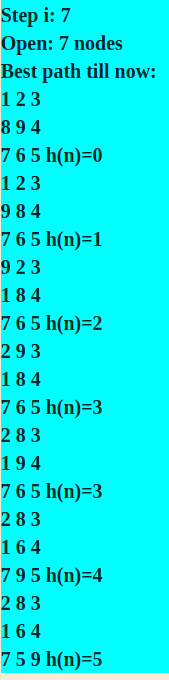
\includegraphics[width=2in, height=7in]{h1.png}
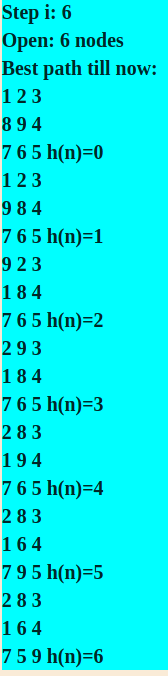
\includegraphics[width=2in, height=7in]{h2.png}
\caption{\label{fig:final}h1 和 h2 的搜索路径结果.}
\end{figure}

在代码中,每一轮生成后继节点后加入对于$f(n) \leq f*(S0)$是否成立的判断,可以验证八数码问题满足该不等式,因此八数码问题使用的是A*算法; 在生成子结点后加入是否满足$h(n_i) \leq 1 + h(n_j)$的判断,则可以验证$h(n)$函数满足单调性。

\subsection{九数码问题}
与八数码问题的代码基本相同,区别在于对两个启发式函数均需要加入对九数码问题中的 0 错放的计算。

但是九数码问题使用相似的启发函数时,虽然得到正确解的路径相同,求解相同问题的搜索图却不相同。如 Figure 2 所示,给定相同初始状态均使用$h1$的搜索路径一致,但由于评估值不同,导致九数码问题需要扩展更多的结点。

\begin{figure}
\centering
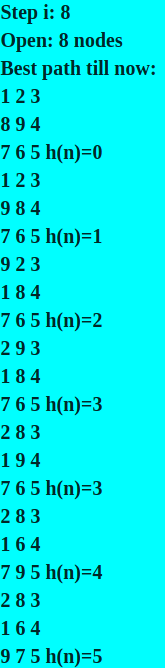
\includegraphics[width=2in, height=7in]{8h1.png}
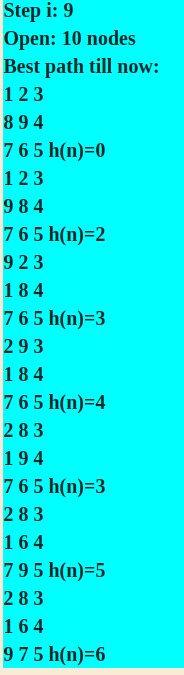
\includegraphics[width=2in, height=7in]{9h1.png}
\caption{\label{fig:final}均使用 h1 时八数码和九数码问题的搜索路径结果.}
\end{figure}


\subsection{其他讨论}
\subsubsection{随机产生初始状态的方法}
由于$h1(n)$函数的启发性较差,对于一些随机生成的八数码情况,可能需要搜索上千甚至上万步才能得到最终解,这不利于我们对于实验结果的观察,因此在打乱时我们采用空格随机向四个方向之一移动有限步的方法生成初始状态。这样做的好处一方面由于相当于是从目标状态逆推,生成的初始状态一定是可达目标状态的,另一方面避免了过多步收敛的问题(测试中通常十几步,最多几百步就能够得到最优解)。

\subsubsection{n数码问题可解的条件}
经查阅相关资料得知,此类问题能够到达目标状态的条件是:初始状态与目标状态的逆序对数同奇偶。\cite{condition} 由于A*算法具有可采纳性,如果问题有解,则A*算法一定能找到最优解。



\section{测试及结论}

八数码问题采用$h1(n)$时的 OPEN 表中结点数和搜索到最优解所需步数一般都较采用$h2(n)$时的多,在问题变得更加复杂(例如那些使用$h1(n)$需要搜索上万次的情况)时, 使用$h2(n)$的优势尤其明显。可以说明$h2(n)$是相比$h1(n)$效率更好的启发函数。这可能是由于$h2(n)$采用了曼哈顿距离计算,可以更好衡量当前状态到目标状态的实际最小费用估计。




\begin{thebibliography}{}
\bibitem{condition} https://blog.csdn.net/u012160954/article/details/50557174
\end{thebibliography}
\end{document}